\documentclass[xcolor=dvipsnames]{beamer}
%\documentclass[handout,xcolor=dvipsnames]{beamer}

% == Packages for beamer
\usepackage{xcolor}
\usepackage{graphicx}
\usepackage{fancybox}
\usepackage{hyperref}
\usepackage{amsmath,amssymb,amsfonts,bm}
\usepackage{wasysym}
\usepackage{colortbl}
\usepackage[english]{babel}
\usepackage{times}
\usepackage[T1]{fontenc}

% == Other Packages
\usepackage{rotating}
\usepackage{latexsym}
\usepackage{ulem}
\usepackage{appendixnumberbeamer}
\usepackage{booktabs}

% == theme & colors
\usetheme{Warsaw}
\usepackage{helvet}
\definecolor{someblue}{rgb}{0,.1,0.8}
\definecolor{dgreen}{rgb}{0,.6,0.8}
\useoutertheme{infolines}

% == New Commands
\newcommand\spacingset[1]{\renewcommand{\baselinestretch}{#1}\small\normalsize}
\renewcommand\r{\right}
\renewcommand\l{\left}
\newcommand\makegaps{\addtolength{\itemsep}{.25\baselineskip}}
\newcommand\makebiggaps{\addtolength{\itemsep}{.5\baselineskip}}

% = For stats & econometrics
\renewcommand{\epsilon}{\varepsilon}
\newcommand\ud{\mathrm{d}}
\newcommand\dist{\buildrel\rm d\over\sim}
\newcommand\ind{\stackrel{\rm indep.}{\sim}}
\newcommand\iid{\stackrel{\rm i.i.d.}{\sim}}
\newcommand\logit{{\rm logit}}
\newcommand\cA{\mathcal{A}}
\newcommand\cN{\mathcal{N}}
\newcommand\E{\mathbb{E}}
\newcommand\V{\mathbb{V}}
\newcommand\cJ{\mathcal{J}}
\newcommand\y{{\bm y}}
\newcommand\Y{{\bm Y}}
\newcommand\X{{\bm X}}
\newcommand\x{{\bm x}}
\newcommand\eps{{\bm\varepsilon}}
\newcommand\zero{{\bm 0}}
\newcommand\be{{\bm\beta}}
\renewcommand\b{{\bm b}}
\newcommand\C{{\bm C}}
\newcommand\D{{\bm D}}
\newcommand\I{{\bm I}}
\newcommand\Z{{\bm Z}}
\newcommand\eeta{{\bm \eta}}
\newcommand{\Var}{\mathrm{Var}}
\newcommand{\Cov}{\mathrm{Cov}}

\DeclareMathOperator*\plim{plim}
\DeclareMathOperator\rank{rank}
\newcommand\indep{\protect\mathpalette{\protect\independenT}{\perp}}
\DeclareMathOperator{\sgn}{sgn}
\def\independenT#1#2{\mathrel{\rlap{$#1#2$}\mkern2mu{#1#2}}}

\newtheorem{assumption}{Assumption}
\newtheorem{iass}{Identification Assumption}
\newtheorem{ires}{Identfication Result}
\newtheorem{estm}{Estimand}
\newtheorem{esti}{Estimator}

\newcommand{\notindep}{{\bot\negthickspace\negthickspace\bot}{\negthinspace
  \negmedspace \negthickspace \negthickspace \diagup
  \;}}
\newcommand{\bs}{\boldsymbol}
\newcommand{\mb}{\mathbf}
\newcommand{\real}{\mathbb{R}}
\renewcommand{\u}{\ensuremath{\mb{u}}}
\renewcommand{\v}{\ensuremath{\mb{v}}}
\newcommand{\U}{\ensuremath{\mb{U}}}
\newcommand{\M}{\ensuremath{\mb{M}}}
\renewcommand{\b}{\ensuremath{\bs{\beta}}}
\newcommand{\e}{\ensuremath{\bs{\epsilon}}}
\newcommand{\bhat}{\ensuremath{\hat{\bs{\beta}}}}
\newcommand{\XX}{\ensuremath{\X'\X}}
\newcommand{\XXinv}{\ensuremath{\left(\XX\right)^{-1}}}
\newcommand{\hatsig}{\ensuremath{\hat{\sigma}^2}}
\newcommand{\sig}{\ensuremath{\sigma^2}}
\newcommand{\hatmat}{\ensuremath{\X \XXinv \X'}}
\newcommand{\ehat}{\ensuremath{\hat{\e}}}
\newcommand{\tr}{\text{tr}}
\newcommand{\Sig}{\ensuremath{\bs{\Sigma}}}
\newcommand{\SigInv}{\ensuremath{\bs{\Sigma^{-1}}}}
\newcommand{\W}{\ensuremath{\mb{W}}}


\title[]{Experiments: Part I}
\subtitle[ ]{PS200C Quant Methods in Politics, Spring 2026}
\author[Hazlett]{Chad Hazlett }
\institute[UCLA]{UCLA\\[1ex]
  \texttt{chazlett@ucla.edu}
}
\date{}

% Auto-outline slides removed

\begin{document}

\begin{frame}
  \titlepage
\end{frame}


\begin{frame}
  \frametitle{Randomization Solves the Selection Problem}
  \small
Recall this formula for the bias of the DIM ($\tilde{\tau}$) relative to ATT:
\begin{eqnarray*}
\tilde{\tau} & = & \E[Y_i|D_i=1]-\E[Y_i|D_i=0] \quad \text{(obs. diff. in means)} \\
 & = & \E[Y_{1i} | D_i=1]-\E[Y_{0i} | D_i=0] \\
 & = & \underbrace{\E[Y_{1i} - Y_{0i} | D_i=1]}_{\tau_{ATT}}
                 +\underbrace{\E[Y_{0i} | D_i=1]-\E[Y_{0i} | D_i=0]}_{\mbox{Bias}}
\end{eqnarray*}
\pause
Stare at the bias term and ask: What could ensure it is zero?
\pause
\medskip

\alert{Random assignment} of $D_i$ will make the treated and untreated units identical on average, such that
$$ \E[Y_{0i}\mid D_i=1] \ = \ \E[Y_{0i}\mid D_i=0] $$

\end{frame}


\begin{frame}{Historical Context}
\small
From ``Experimentation and social interventions: a forgotten but important history'' (Ann Oakley, 1998, \textit{BMJ}). From the summary points:

\footnotesize
\begin{itemize}

\item<1-> Many social scientists argue that randomised controlled trials are inappropriate for evaluating social interventions, but they ignore a considerable history, mainly in the United States, of the use of randomised controlled trials to assess different approaches to public policy and health promotion

\item<2-> A tradition of experimental sociology was well established by the 1930s, built on the early use of controlled experiments in psychology and education

\item<3-> From the early 1960s to early 1980s randomised experiments were considered the optimal design for evaluating public policy interventions in the United States, and major evaluations using this design were carried out.\footnote{Also note Campbell \& Stanley published ``Experimental and Quasi-experimental designs for research'' in 1966}

\item<4-> This approach became less popular as policy makers reacted negatively to evidence of ``near zero'' effects

\item<5-> Lessons to be learnt about implementing randomised controlled trials in real life settings include the difficulty of assessing complex multi-level interventions and the challenge of integrating qualitative data

\end{itemize}
\end{frame}


\begin{frame}
  \frametitle{Re-rise of experiments}
\small
\onslide<1->  Though much of the history forgotten, renewed enthusiasm and ``rediscovery'' of experiments for social sciences early this century
\begin{itemize}
  \item {\it Abbreviated} list of examples (from Green 2008):
  \begin{itemize}
  \addtolength{\itemsep}{.25\baselineskip}
  \smallskip
  \footnotesize
    \item \alert{Program evaluation}: development programs, education programs, SAT prep classes, weight loss programs,  diversity training, deliberative polls, advertising campaigns, website designs...
    \item \alert{Public policy evaluation}: teacher pay, student incentives, class size,
      speed traps, vouchers, alternative sentencing, job training,
      health insurance subsidies, tax compliance, public housing
    \item \alert{Behavioral research}: persuasion, mobilization, education, income, interpersonal influence, conscientious health behaviors, media exposure, deliberation, discrimination
    \item \alert{Research on institutions}: transparency, corruption, electoral systems, information
  \end{itemize}
  \item Also 2019 Nobel prize in economics.
\end{itemize}

\end{frame}


\section{Identification}

\begin{frame}
  \frametitle{Identification vs. Estimation}
  \small
Goal of causal inference: Learn about an \textit{unobservable, counterfactual-dependent} quantity of interest (QoI) using {\it observed} data.\\

\pause

\medskip
Two inferential hurdles:

\begin{enumerate}
\item \alert{Identification}: If you can observe data from an entire {\it population}, can you learn about your QoI?
\item \alert{Estimation}: Given your finite amount of data on a {\it sample}, how well can you learn about your QoI?
\end{enumerate}
\pause
\begin{center}
Golden rule of inference: \textbf{Identification precedes estimation}
\end{center}
\end{frame}


\begin{frame}{The Template}
Before we say more about experiments, take note of the general template for talking about an identification strategy; we will repeat it through the remainder of the course. \\

\bigskip
\onslide<2-> We organize our thinking about how to make causal claims by \textcolor{blue}{identification strategy}.\\

\bigskip

\onslide<3-> For each we discuss:\\
\small
\begin{enumerate}
\item  the \textcolor{blue}{identification assumption} first, which your life will depend upon when using this approach.
\item information from outside the data that help support that assumption
\item the (limited) things you can test in efforts to falsify the assumption
\item estimators
\item ideally, sensitivity to violations of assumptions
\end{enumerate}
\end{frame}


%%%%%%%%% frame %%%%%%%%%
\begin{frame}
\frametitle{Classical Randomized Experiment}
\small
Setup:
\begin{itemize}
\item Units: $i = 1, ..., N$
\item Treatment: $D_i \in \{0,1\}$, randomly assigned
\item Potential outcomes: $Y_{0i}$, $Y_{1i}$
\item Observed outcome: $Y_i = Y_{D_i{i}}$
\item Number of treated/untreated units: $N_1 = \sum_{i=1}^N D_i$ and $N_0 = N - N_1$
\end{itemize}

\pause
Notes:
\footnotesize
\begin{itemize}
\item Random assignment can take one of several forms:
	\begin{itemize}
	\scriptsize
	\makegaps
	\item \alert{Complete randomization}: Exactly $N_1$ treated units
	\item \alert{Simple (Bernoulli) randomization}: Each unit independently assigned to treatment with probability $p$
	\end{itemize}
\end{itemize}

\end{frame}


\begin{frame}[t]
\frametitle{Identification of Average Treatment Effect Under Experiments}
\small
\onslide<1-> \textcolor{Blue}{Identification Assumption}: (guaranteed by random assignment):
$$ \l\{ Y_{1i}, \ Y_{0i}\r\} \ \indep \ D_i $$ \\

\onslide<2-> \textcolor{Blue}{Quantity of Interest}: \\
\vspace{-.2in}
$$ \tau_{ATE} \ \equiv \ \E[Y_{1i} - Y_{0i}]$$
\onslide<3-> \textcolor{Blue}{How does our ID assumption lead to identification of $\tau_{ATE}$}?\\
\footnotesize
\onslide<4-> \begin{eqnarray*}
\E[Y_{1i}] - \E[Y_{0i}] &=& \E[Y_{1i}|D_i=1] - \E[Y_{0i} | D_i=0] \quad (\text{why?}) \\
&=& \E[Y_{i}|D_i=1] - \E[Y_{i} | D_i=0]  \quad (\text{why?})\\
&=& \text{DIM Estimand}\\
&\approx & \overline{Y}_1 - \overline{Y}_0   \quad (\text{the DIM estimator})
\end{eqnarray*}
\end{frame}


\section{Estimation and Inference}

\begin{frame}{SATE and PATE}
\begin{itemize}
\itemsep1pt\parskip0pt\parsep0pt
\item<1->
 Often we focus on estimating the average causal effect in a
  particular sample: \textbf{S}ample \textbf{A}verage \textbf{T}reatment
  \textbf{E}ffect (SATE)\medskip

  \begin{itemize}
   \item uncertainty arises only from hypothetical randomizations.\medskip
  \item  inferences are limited to the sample in our study.
  \end{itemize}\bigskip
\item<2-> Compare to the \textbf{P}opulation
  \textbf{A}verage \textbf{T}reatment \textbf{E}ffect (PATE)\medskip
 \begin{itemize}
  \item Imagines uncertainty in both the sample drawn from the (larger) population, and in treatment assignment.
  \end{itemize}\bigskip


\item<3->  \small  If your sampling was random from a given population, then $\E[SATE]=PATE$. For this reason, we're often uninterested in distinguishing the two quantities.
\end{itemize}
\end{frame}


\begin{frame}{Standard Errors for the ATE}
\small
\onslide<1-> Variance of the difference in means estimator:
\begin{align*}
\V({\overline{Y}_1 -\overline{Y}_0}) &= \frac{\sigma^2_{Y1}}{N_1} + \frac{\sigma^2_{Y0}}{N_0}
\end{align*}
where $\sigma^2_{Y1}$ and $\sigma^2_{Y0}$ are the variance of the $Y_{1i}$ and $Y_{0i}$ in the population.\\

\medskip
\onslide<2-> The Neyman estimator:
\begin{align*}
\widehat{SE}_{ATE} &= \sqrt{\frac{\hat{\sigma}^2_{Y1}}{N_1} + \frac{\hat{\sigma}^2_{Y0}}{N_0}}
\end{align*}

\onslide<3-> Key facts:
\begin{itemize}
\footnotesize
\item This is the correct SE for the \textbf{PATE}
\item It is what you get from t-tests (unequal variance), or regression with robust SE
\item It is \textbf{conservative} for the \textbf{SATE} (proof in appendix)
\end{itemize}
\end{frame}


\begin{frame}
  \frametitle{Example: Effect of Training on Earnings}
\small
\begin{itemize}
  \item Treatment Group:
  \begin{itemize}
  \item $N_1=7,487$
    \item Estimated Average Earnings $\bar{Y}_1$: \$$16,199$
    \item Estimated Sample Standard deviation $\widehat{\sigma}_{Y|D_i=1}$: $\$17,038$
  \end{itemize}\smallskip

  \item Control Group :
  \begin{itemize}
  \item $N_0=3,717$
    \item Estimated Average Earnings $\bar{Y}_0$: \$$15,040$
    \item Estimated Sample  deviation $\widehat{\sigma}_{Y|D_i=0}$: $\$16,180$
  \end{itemize}\smallskip
  \item Estimated average effect of training: \pause
  \begin{itemize}
    \item $\widehat{\tau}_{ATE} = \bar{Y}_1 - \bar{Y}_0 = 16,199 - 15,040 = \$1,159$
  \end{itemize}\smallskip
  \item Estimated standard error for effect of training: \pause
\scriptsize
$$\widehat{ SE}_{\widehat{ATE}} = \sqrt{ \frac{ \widehat{\sigma}^2_{Y|D_i=1}  }{N_1}+ \frac{ \widehat{\sigma}^2_{Y|D_i=0} }{N_0}} = \sqrt{\frac{17,038^2}{7,487}+ \frac{16,180^2}{3,717} }\approx\$330$$
\small
  \item Is this consistent with a zero average treatment effect $\alpha_{ATE}=0$?
\end{itemize}

\end{frame}


\begin{frame}
  \frametitle{Testing the Null Hypothesis of Zero Average Effect}
\small
\onslide<1-> \textcolor{Blue}{Null hypothesis, H$_0$}: $\tau_{ATE}=0$\\
\bigskip
\onslide<2-> We observe a difference in mean earnings of $\hat{\tau}_{ATE}=1,159$ \\
\bigskip
\onslide<3-> Would it be surprising to see such an estimate had the null been true? \\
\footnotesize
\begin{itemize}
\item<4-> you likely know already:
\item<5-> 1,159 is more than 2 SEs from 0, so you know $t$-stat/ $z$-score would be over 2 and p-value would be less than 0.05.
\smallskip
\item<6-> to recall the formalities,
\end{itemize}
\end{frame}


\begin{frame}[fragile]
\frametitle{Testing the Null Hypothesis of Zero Average Effect}
\small
\onslide<1-> Use a two-sample t (or z) test with unequal variances:\[
t=\frac{\widehat{\tau}}{\sqrt{\displaystyle\frac{\widehat{\sigma}_{Y_i|D_i=1}^2}{N_1} + \displaystyle\frac{\widehat{\sigma}_{Y_i|D_i=0}^2}{N_0}}}=\frac{\$1,159}{\sqrt{\displaystyle\frac{\$17,038^2}{7,487} + \displaystyle\frac{\$16,180^2}{3,717}}}\approx3.5
\]
\begin{itemize}
\footnotesize
\item For large enough $N$, $t \stackrel{d}{\rightarrow} N(0,1)$,
\item Getting a 3.5 or above from a normal distribution would be quite a shock:
\scriptsize
\begin{verbatim}
> 2*(1-pnorm(abs(3.5)))
[1] 0.000465
\end{verbatim}
\footnotesize
\item Inverting the test statistic we can construct a 95\% confidence interval
\[
\widehat{\tau}_{ATE}\pm 1.96 \cdot \widehat{ SE}_{\widehat{ATE}}
\]
\item What assumptions did we need along the way?
\end{itemize}
\end{frame}


\begin{frame}[fragile]
\frametitle{Testing the Null Hypothesis of Zero Average Effect}
{
\footnotesize
\begin{Verbatim}[frame=single, label=R Code, commandchars=\\\{\}]
> d <- read.dta("jtpa.dta")
> t.test(earnings~assignmt,data=d,var.equal=FALSE)

	Welch Two Sample t-test

data:  earnings by assignmt
t = -3.5084, df = 7765.599, p-value = 0.0004533
alternative hypothesis: true difference in means is not equal to 0
95 percent confidence interval:
 -1807.2427  -511.6239
sample estimates:
mean in group 0 mean in group 1
       15040.50        16199.94
\end{Verbatim}
}
\end{frame}


\begin{frame}
  \frametitle{Regression to Estimate ATE in Experiments}
\small
\begin{esti}[Regression with Experiments]\small
The ATE can be expressed as a regression coefficient:
\begin{eqnarray*}
  Y_i &=& D_i\, Y_{1i} + (1-D_i)\, Y_{0i} \\
   &=& Y_{0i} + (Y_{1i}- Y_{0i})\,D_i \\
   &=& \underbrace{\bar Y_0}_{\alpha} + \underbrace{(\bar Y_1 - \bar Y_0)}_{\tau_{Reg}} D_i + \underbrace{\{(Y_{i0} - \bar Y_0) + D_i \cdot [(Y_{i1} - \bar Y_1) - (Y_{i0} - \bar Y_0)] \}}_{\epsilon} \\
   &=& \alpha + \tau_{Reg} D_i + \epsilon_i
\end{eqnarray*}
\end{esti}\vspace{-.2in}
\bigskip
\begin{itemize}
\footnotesize
\item<2-> Does this assume constant treatment effects?
\item<3-> Our SE estimator allows different variance for $D=1$ and $D=0$.
  \begin{itemize}
\scriptsize
  \item  Implies heteroskedasticity
  \item Use ``HC2'' heteroskedasticity-robust variance:
  $$ \hat\sigma^2_{HC2} \ = \ \frac{S_1^2}{N_1} + \frac{S_0^2}{N_0} \ = \ \tilde{\V}(\tilde\tau) $$
  \end{itemize}
\end{itemize}
\end{frame}


\begin{frame}[fragile]
\frametitle{Regression to Estimate the Average Treatment Effect}
{
\footnotesize
\begin{Verbatim}[frame=single, label=R Code, commandchars=\\\{\}]
> library(sandwich)
> library(lmtest)
>
> lout <- lm(earnings~assignmt,data=d)
> coeftest(lout,vcov = vcovHC(lout, type = "HC2"))

t test of coefficients:

            Estimate Std. Error t value  Pr(>|t|)
(Intercept) 15040.50     265.38 56.6752 < 2.2e-16 ***
assignmt     1159.43     330.46  3.5085 0.0004524 ***
---
\end{Verbatim}
}
\end{frame}


\section{Randomization Inference}

\begin{frame}\frametitle{Testing in Small Samples: Fisher's Exact Test}
\begin{itemize}
\item Test of differences in means with large $N$:
\small
\[
H_0:\E[Y_1] =\E[Y_0],\quad H_1:\E[Y_1] \neq\E[Y_0]  \mbox{  (weak null)}
\]\pause
\normalsize
\item Fisher's Exact Test:
\small
\[
H_0: Y_{1i} = Y_{0i},\pause\quad H_1: Y_1 \neq Y_0\;\; \forall i,\;\;\qquad\mbox{(sharp null of no effect)}
\]\pause
\end{itemize}
\normalsize
\vspace{-.2in}
\onslide<4-> \alert{Key idea}: Under the sharp null, we ``observe'' all potential outcomes -- can compute what ATE would be under alternate randomizations \\
\pause
\medskip
...which allows you to see many effect estimates all under this null.
\end{frame}


\begin{frame}\frametitle{Testing in Small Samples: Fisher's Exact Test}
\small
\onslide<1-> Let $\Omega$ be the set of all possible ways to assign treatments. \\
\bigskip
\onslide<2-> Fisher's exact test procedure:\\
\footnotesize
\begin{enumerate}
\item<3->  Calculate a statistic $\hat{\theta}_{true}$ (e.g. difference in means) from original treatment assignment data
\item<4->  Obtain the null distribution of the statistic by calculating the same statistic $\hat{\theta}(\omega)$ under the sharp null for every possible (or many) $\omega$ in $\Omega$
\item<5-> Compare $\hat{\theta}_{true}$ to the null distribution of $\hat{\theta}(\omega)$'s to see how ``extreme'' it is
\end{enumerate}
\end{frame}


% -- Slide 1: The setup with missing POs --
\begin{frame}
\frametitle{Fisher's Exact Test: Setup}
\smallskip
\begin{tabular}{@{} c c c c @{}}
\toprule
$i$ & $Y_{1i}$ & $Y_{0i}$ & $D_i$ \\
\midrule
\rowcolor{blue!8}  1 & 3 & \textcolor{red!70!black}{?} & 1 \\
\rowcolor{blue!8}  2 & 1 & \textcolor{red!70!black}{?} & 1 \\
                    3 & \textcolor{red!70!black}{?} & 0 & 0 \\
                    4 & \textcolor{red!70!black}{?} & 1 & 0 \\
\midrule
$\widehat{\tau}_{\text{ATE}}$ & & & 1.5 \\
\bottomrule
\end{tabular}
\bigskip\\
What do we know given the sharp null $H_0: Y_{1i} = Y_{0i}$?
\end{frame}

% -- Slide 2: Sharp null fills in all POs --
\begin{frame}
\frametitle{Fisher's Exact Test: Sharp Null Fills In POs}
\smallskip
\begin{tabular}{@{} c c c c @{}}
\toprule
$i$ & $Y_{1i}$ & $Y_{0i}$ & $D_i$ \\
\midrule
\rowcolor{blue!8}  1 & 3 & \textcolor{red!70!black}{3} & 1 \\
\rowcolor{blue!8}  2 & 1 & \textcolor{red!70!black}{1} & 1 \\
                    3 & \textcolor{red!70!black}{0} & 0 & 0 \\
                    4 & \textcolor{red!70!black}{1} & 1 & 0 \\
\midrule
$\widehat{\tau}_{\text{ATE}}$ & & & 1.5 \\
$\hat\tau(\omega)$ & & & 1.5 \\
\bottomrule
\end{tabular}
\bigskip\\
\small
Given the full schedule of potential outcomes under the sharp null, we can compute the null distribution of the ATE across all possible randomizations.
\end{frame}

% -- Slide 3: Building up alternative randomizations --
\begin{frame}
\frametitle{Fisher's Exact Test: First Alternative Randomization}
\smallskip
\begin{tabular}{@{} c c c c !{\color{gray!50}\vrule} c @{}}
\toprule
$i$ & $Y_{1i}$ & $Y_{0i}$ & $D_i$ & $\omega_1$ \\
\midrule
\rowcolor{blue!8}  1 & 3 & \textcolor{red!70!black}{3} & 1 & 1 \\
                    2 & 1 & \textcolor{red!70!black}{1} & 1 & 0 \\
\rowcolor{blue!8}  3 & \textcolor{red!70!black}{0} & 0 & 0 & 1 \\
                    4 & \textcolor{red!70!black}{1} & 1 & 0 & 0 \\
\midrule
$\widehat{\tau}_{\text{ATE}}$ & & & 1.5 &  \\
$\hat\tau(\omega)$ & & & 1.5 & 0.5 \\
\bottomrule
\end{tabular}
\end{frame}

\begin{frame}
\frametitle{Fisher's Exact Test: Adding Randomizations}
\smallskip
\begin{tabular}{@{} c c c c !{\color{gray!50}\vrule} c c @{}}
\toprule
$i$ & $Y_{1i}$ & $Y_{0i}$ & $D_i$ & $\omega_1$ & $\omega_2$ \\
\midrule
\rowcolor{blue!8}  1 & 3 & \textcolor{red!70!black}{3} & 1 & 1 & 1 \\
                    2 & 1 & \textcolor{red!70!black}{1} & 1 & 0 & 0 \\
                    3 & \textcolor{red!70!black}{0} & 0 & 0 & 1 & 0 \\
\rowcolor{blue!8}  4 & \textcolor{red!70!black}{1} & 1 & 0 & 0 & 1 \\
\midrule
$\widehat{\tau}_{\text{ATE}}$ & & & 1.5 &  &  \\
$\hat\tau(\omega)$ & & & 1.5 & 0.5 & 1.5 \\
\bottomrule
\end{tabular}
\end{frame}

\begin{frame}
\frametitle{Fisher's Exact Test: Adding Randomizations}
\smallskip
\begin{tabular}{@{} c c c c !{\color{gray!50}\vrule} c c c @{}}
\toprule
$i$ & $Y_{1i}$ & $Y_{0i}$ & $D_i$ & $\omega_1$ & $\omega_2$ & $\omega_3$ \\
\midrule
                    1 & 3 & \textcolor{red!70!black}{3} & 1 & 1 & 1 & 0 \\
\rowcolor{blue!8}  2 & 1 & \textcolor{red!70!black}{1} & 1 & 0 & 0 & 1 \\
\rowcolor{blue!8}  3 & \textcolor{red!70!black}{0} & 0 & 0 & 1 & 0 & 1 \\
                    4 & \textcolor{red!70!black}{1} & 1 & 0 & 0 & 1 & 0 \\
\midrule
$\widehat{\tau}_{\text{ATE}}$ & & & 1.5 & & & \\
$\hat\tau(\omega)$ & & & 1.5 & 0.5 & 1.5 & $-1.5$ \\
\bottomrule
\end{tabular}
\end{frame}

\begin{frame}
\frametitle{Fisher's Exact Test: Adding Randomizations}
\smallskip
\begin{tabular}{@{} c c c c !{\color{gray!50}\vrule} c c c c @{}}
\toprule
$i$ & $Y_{1i}$ & $Y_{0i}$ & $D_i$ & $\omega_1$ & $\omega_2$ & $\omega_3$ & $\omega_4$ \\
\midrule
                    1 & 3 & \textcolor{red!70!black}{3} & 1 & 1 & 1 & 0 & 0 \\
\rowcolor{blue!8}  2 & 1 & \textcolor{red!70!black}{1} & 1 & 0 & 0 & 1 & 1 \\
                    3 & \textcolor{red!70!black}{0} & 0 & 0 & 1 & 0 & 1 & 0 \\
\rowcolor{blue!8}  4 & \textcolor{red!70!black}{1} & 1 & 0 & 0 & 1 & 0 & 1 \\
\midrule
$\widehat{\tau}_{\text{ATE}}$ & & & 1.5 & & & & \\
$\hat\tau(\omega)$ & & & 1.5 & 0.5 & 1.5 & $-1.5$ & $-0.5$ \\
\bottomrule
\end{tabular}
\end{frame}

% -- Complete table with p-value --
\begin{frame}
\frametitle{Fisher's Exact Test: All Randomizations}
\smallskip
\begin{tabular}{@{} c c c c !{\color{gray!50}\vrule} c c c c c @{}}
\toprule
$i$ & $Y_{1i}$ & $Y_{0i}$ & $D_i$ & $\omega_1$ & $\omega_2$ & $\omega_3$ & $\omega_4$ & $\omega_5$ \\
\midrule
                    1 & 3 & \textcolor{red!70!black}{3} & 1 & 1 & 1 & 0 & 0 & 0 \\
                    2 & 1 & \textcolor{red!70!black}{1} & 1 & 0 & 0 & 1 & 1 & 0 \\
\rowcolor{blue!8}  3 & \textcolor{red!70!black}{0} & 0 & 0 & 1 & 0 & 1 & 0 & 1 \\
\rowcolor{blue!8}  4 & \textcolor{red!70!black}{1} & 1 & 0 & 0 & 1 & 0 & 1 & 1 \\
\midrule
$\widehat{\tau}_{\text{ATE}}$ & & & 1.5 & & & & & \\
$\hat\tau(\omega)$ & & & 1.5 & 0.5 & 1.5 & $-1.5$ & $-0.5$ & $-1.5$ \\
\bottomrule
\end{tabular}
\vspace{.2in}\\
So \textit{under null}: $\Pr\!\bigl(|\hat\tau(\omega)| \geq |\widehat{\tau}_{\text{ATE}}|\bigr)=4/6\approx.67$.
\end{frame}


\begin{frame}{Scaling Up}
\small
With 4 units and 2 treated, there are only $\binom{4}{2}=6$ possible assignments --- we can enumerate them all.\\
\bigskip
\onslide<2-> With 50 units and 25 treated, there are $\binom{50}{25} \approx 1.26 \times 10^{14}$ possible assignments.\\
\bigskip
\onslide<3-> We can't enumerate --- but we can \alert{sample} from $\Omega$.\\
\medskip
\begin{itemize}
\item<3-> Randomly re-assign treatment many times (e.g.\ 10,000)
\item<4-> Compute $\hat\tau(\omega)$ each time under the sharp null
\item<5-> This gives us the \textbf{null distribution} of the test statistic
\item<6-> Compare our observed $\hat\tau$ to this distribution
\end{itemize}
\end{frame}


\begin{frame}{Randomization Inference in Practice}
\vspace{-.5cm}
\begin{center}
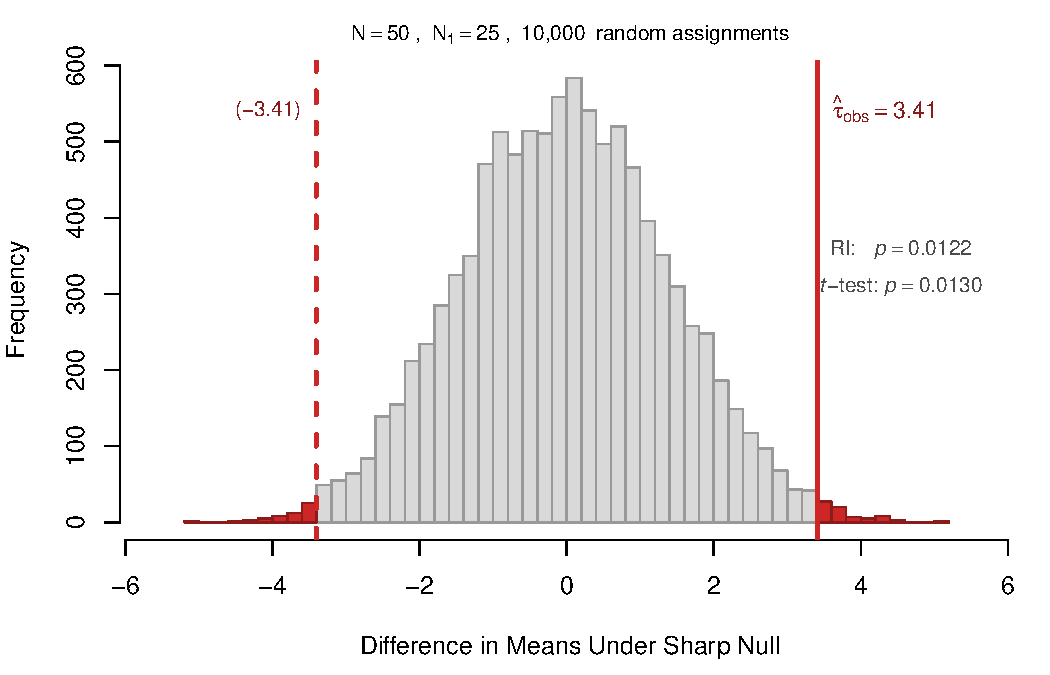
\includegraphics[width=.8\linewidth]{images/ri_null_distribution.pdf}
\end{center}
\vspace{-.2cm}
\footnotesize
\onslide<2-> Histogram: 10,000 sampled re-randomizations under sharp null.\\
Solid line: observed $\hat\tau$. Shaded regions: values at least as extreme $\Rightarrow$ p-value.
\end{frame}


\begin{frame}{How do these inferences differ?}
\small
\onslide<1-> \textbf{Finite-sample exactness.} \\
\footnotesize
\begin{itemize} 
\item<1-> The Fisher/RI p-value is exact under the sharp null --- no appeal to large-$N$ approximations (CLT).
\item<1-> When $N$ is large enough for the CLT, the null distribution looks normal and you get nearly the same answer as a $t$-test (as we saw)
\end{itemize}
\medskip
\onslide<2-> \textbf{The sharp null is a strong hypothesis}: $Y_{1i} = Y_{0i}$ for \textit{every} unit.\\
\footnotesize
\begin{itemize}
\item<3-> But any summary test statistic (DIM, rank statistic, etc.)\ is only sensitive to effects that accumulate --- not to effects that cancel. In practice, rejecting the sharp null via the DIM tells ``effects exist \textit{and} don't average to zero'', similar to weak null.
\end{itemize}
\small
\onslide<4-> \textbf{Compare to the bootstrap}\\
\footnotesize
\begin{itemize}
\item The bootstrap resamples \textit{units} --- simulating ``what if we'd drawn different people from the population?'' Reflects super-population uncertainty. 
\item RI is ``design-based'' -- re-randomizes \textit{treatment assignment} within the fixed sample --- ``what same people received different treatment assignment?''\
\end{itemize}
\small
\onslide<5-> \textbf{Bottom line}: RI valuable in \alert{small samples} where normality is a worry.
\end{frame}


%% ============================================================
%%  APPENDIX
%% ============================================================

\appendix

\begin{frame}
\begin{center}
\Large Appendix
\end{center}
\end{frame}

%% --- Neyman SE is conservative for SATE ---

%% --- A1: Neyman SE is conservative for SATE ---

\begin{frame}
\frametitle{The exact SE for SATE}
\small
\onslide<1-> In reality we can only assign treatment within a finite sample so expect $cov(\overline{Y}_1,\overline{Y}_0) \neq 0$.\\

\medskip
\onslide<2-> Considering this, under complete randomization the true standard error of the sample ATE is actually
\pause
\footnotesize
 \begin{eqnarray*}
 SE_{\widehat{ATE}}&=&\sqrt{ \left( \frac{N-N_1}{N-1}\right) \frac{\sigma^2_{Y1}}{N_1}+ \left( \frac{N-N_0}{N-1}\right) \frac{\sigma^2_{Y0}}{N_0} + \left(\frac{1}{N-1} \right) 2Cov[Y_{1},Y_{0}]} \\
\end{eqnarray*}
\vspace{-.1in}
\small
with population variances and covariances $\sigma^2_{Yd}$, $Cov(Y_{1},Y_{0})$.\\
\bigskip

\onslide<3-> We don't use this---can you see why?
\end{frame}


\begin{frame}{Proof that Neyman SE is conservative for SATE}
\small
Two preliminaries:
\footnotesize
\begin{itemize}
\item $Cov(Y_1,Y_0) \leq SD(Y_1)SD(Y_0)$
\item $Var(Y_1) + Var(Y_0) \geq 2\sqrt{Var(Y_1) Var(Y_0)}$
\end{itemize}
\small
\onslide<2-> With that,
\scriptsize
\begin{eqnarray*}
  SE_{\widehat{ATE}}  & = & \sqrt{ \left( \frac{N-N_1}{N-1}\right) \frac{Var[Y_{1}]}{N_1}+ \left( \frac{N-N_0}{N-1}\right) \frac{Var[Y_{0}]}{N_0} + \left(\frac{1}{N-1} \right) 2Cov[Y_{1},Y_{0}]} \\
 & = & \sqrt{ \frac{1}{N-1} \left(\frac{N_0}{N_1}Var[Y_1]+\frac{N_1}{N_0}Var[Y_0]+2Cov[Y_1,Y_0]\right)}  \\
                      & \leq & \sqrt{\frac{1}{N-1}\left( \frac{N_0}{N_1}Var[Y_1]+\frac{N_1}{N_0}Var[Y_0] +2\sqrt{Var[Y_1]Var[Y_0]}\right)} \\
                     & \leq & \sqrt{\frac{1}{N-1}\left( \frac{N_0}{N_1}Var[Y_1]+\frac{N_1}{N_0}Var[Y_0]  + Var[Y_1]+Var[Y_0]\right)} \\
\end{eqnarray*}
\end{frame}


\begin{frame}
  \frametitle{$SE_{\widehat{ATE}}\leq \widehat{SE}_{\widehat{ATE}}$, continued.}
\scriptsize
\begin{eqnarray*}
\scriptsize
  SE_{\widehat{ATE}} & \leq &\sqrt{\frac{1}{N-1}\left( \frac{N_0}{N_1}Var[Y_1]+\frac{N_1}{N_0}Var[Y_0]  + Var[Y_1]+Var[Y_0]\right)} \\
  & \leq & \sqrt{ \frac{N_0^2Var[Y_1]+N_1^2 Var[Y_0] + N_1 N_0 (Var[Y_1]+Var[Y_0])}{(N-1)N_1 N_0}} \\
  & \leq & \sqrt{ \frac{(N_0^2 + N_1 N_0) Var[Y_1]+(N_1^2 + N_1 N_0) Var[Y_0] }{(N-1)N_1 N_0}} \\
    & \leq & \sqrt{ \frac{(N_0 + N_1) N_0 Var[Y_1]}{(N-1) N_1 N_0}+ \frac{ (N_1 + N_0) N_1  Var[Y_0]}{(N-1)N_1 N_0}}  \\
    & \leq & \sqrt{ \frac{N \,  Var[Y_1]}{(N-1) N_1 }+ \frac{ N \, Var[Y_0]}{(N-1) N_0}}  \\
    & \leq & \sqrt{\frac{N}{N-1} \left(\frac{Var[Y_1]}{N_1}+ \frac{ Var[Y_0]}{(N_0)}\right)}  \\
    &\leq & \sqrt{ \left(\frac{Var[Y_1]}{N_1}+ \frac{ Var[Y_0]}{(N_0)}\right)}
\end{eqnarray*}
\small
$\therefore$ our estimator is conservative.
\end{frame}


\end{document}
